%%%%%%%%%%%%%%%%%%%%%%%%%%%%%%%%%%%%%%%%%%%%%%%%%%%%%%%%%%%%%%%%%%%%%%%%
%    INSTITUTE OF PHYSICS PUBLISHING                                   %
%                                                                      %
%   `Preparing an article for publication in an Institute of Physics   %
%    Publishing journal using LaTeX'                                   %
%                                                                      %
%    LaTeX source code `ioplau2e.tex' used to generate `author         %
%    guidelines', the documentation explaining and demonstrating use   %
%    of the Institute of Physics Publishing LaTeX preprint files       %
%    `iopart.cls, iopart12.clo and iopart10.clo'.                      %
%                                                                      %
%    `ioplau2e.tex' itself uses LaTeX with `iopart.cls'                %
%                                                                      %
%%%%%%%%%%%%%%%%%%%%%%%%%%%%%%%%%%
%
%
% First we have a character check
%
% ! exclamation mark    " double quote  
% # hash                ` opening quote (grave)
% & ampersand           ' closing quote (acute)
% $ dollar              % percent       
% ( open parenthesis    ) close paren.  
% - hyphen              = equals sign
% | vertical bar        ~ tilde         
% @ at sign             _ underscore
% { open curly brace    } close curly   
% [ open square         ] close square bracket
% + plus sign           ; semi-colon    
% * asterisk            : colon
% < open angle bracket  > close angle   
% , comma               . full stop
% ? question mark       / forward slash 
% \ backslash           ^ circumflex
%
% ABCDEFGHIJKLMNOPQRSTUVWXYZ 
% abcdefghijklmnopqrstuvwxyz 
% 1234567890
%
%%%%%%%%%%%%%%%%%%%%%%%%%%%%%%%%%%%%%%%%%%%%%%%%%%%%%%%%%%%%%%%%%%%
%
\documentclass[12pt]{iopart}
\usepackage{xcolor}
\usepackage{pifont}
\usepackage{comment}
%\usepackage{subcaption}
\usepackage{tikz}
\usetikzlibrary{shapes.geometric, arrows, calc}
\expandafter\let\csname equation*\endcsname\relax 
\expandafter\let\csname endequation*\endcsname\relax 
\usepackage{amsmath}
\usepackage{amssymb}
\newcommand{\gguide}{{\it Preparing graphics for IOP Publishing journals}}
%Uncomment next line if AMS fonts required
%\usepackage{iopams}  
\newcommand{\jordan}[1]{\textbf{\textcolor{red}{JORDAN: #1}}}
\newcommand{\siong}[1]{\textbf{\textcolor{blue}{SIONG: #1}}}
\newcommand{\chris}[1]{\textbf{\textcolor{green}{CHRIS: #1}}}
\newcommand{\michael}[1]{\textbf{\textcolor{orange}{MICHAEL: #1}}}
\begin{document}

\title{Generative Adversarial Networks and Gravitational Waves}

\author{J. McGinn}

\address{University of Glasgow, Physics \& Astronomy Department, Glasgow G12 8QQ, UK}
%\ead{jordan.mcginn@glasgow.ac.uk}
\vspace{10pt}
\begin{indented}
\item[]March 2020
\end{indented}

\begin{abstract}

\end{abstract}

%
% Uncomment for keywords
%\vspace{2pc}
%\noindent{\it Keywords}: XXXXXX, YYYYYYYY, ZZZZZZZZZ
%
% Uncomment for Submitted to journal title message
%\submitto{\JPA}
%
% Uncomment if a separate title page is required
%\maketitle
% 
% For two-column output uncomment the next line and choose [10pt] rather than [12pt] in the \documentclass declaration
%\ioptwocol
%



\section{Introduction}
\begin{itemize}
\item Need to introduce GWs - the current state of the field e.g. detections
and LVC papers \ding{51}
\item Introduce burst searches - what's the point of burst searches \ding{51} - lots of references 
\item Discuss the family of burst waveforms currently used and why - not in detail, just
an introduction \ding{51}
\item Introduce ML techniques in GWs \ding{51} - lots of references
\item What this paper does on GANs in 1 paragraph \ding{51}
\item Describe the structure of the paper 
\end{itemize}

Gravitational-wave (GW) astronomy is now an established field, starting with the first detection of a binary black hole merger \cite{} on September 2015. Following this, the first and second observations runs (O1 and O2) of Advanced LIGO and Advanced Virgo reported several more mergers \cite{}. On August 2017 a binary neutron star merger was observed alongside its electron-magnetic counterpart for the first time, giving rise to multimessenger gravitational wave astronomy. 
GW bursts are transient signals of typically short duration ($<$ 1s) whose waveforms are not accurately modelled or are complex to re-produce. Astrophysical sources for such transients include: \jordan{should i include a list of these?}. Since GW bursts are un-modelled they are not sensitive to template based detection schemes such as matched-filtering \cite{}, instead, detection involves distinguishing the signal from detector noise. This is only possible if the detector noise is well characterised and the candidate signal can be differentiated from system or environmental glitches. As such, GW burst searches rely on an astrophysical burst signature appearing in multiple detectors. \jordan{how deep should i go? with coherent WaveBurst etc?}
Many GW burst algorithms \cite{cite the shit outta this} are tested and tuned using model waveforms that may or may not have astrophysical significance but have easy to define parameters and share characteristics of real bursts that is enough to simulate coincident non-stationary deviations between detectors. Such waveforms may have long-duration, short bandwidth (ringdowns), long-duration, large bandwidth (inspirals) and many algorithms make use of sine-Gaussians: a Gaussian modulated sine wave that is characterised by it's central frequency and narrow bandwidth. This makes it a great tool for diagnosing LIGOs sensitivity to frequency. 
We aim to explore the use of machine learning in generating and interpreting these mock GW burst signals. Neural networks have shown to replicate the sensitivities of matched filtering in GW detection \cite{} and rapid parameter estimation \cite{}, however these methods have primarily been focused on binary black hole signals and have not yet expanded to burst examples. 

%%%%%%%%%%%%%%%%%%%%%%%%%%%%%%%%%%%%%%%%%%%%%%%%%%%%%%%%%%%%%%%%%%%%%%%%%%%%%%
\section{Generative Adversarial Networks}
%%%%%%%%%%%%%%%%%%%%%%%%%%%%%%%%%%%%%%%%%%%%%%%%%%%%%%%%%%%%%%%%%%%%%%%%%%%%%%

\begin{itemize}
\item Describe GANs in detail but really focus on the fact that the reader is a
GW data analyst - not a computer scientist \ding{51}
\item A diagram would be very useful \ding{51}
\item Do not discuss our specific case here - just stay general \ding{51}
\item A subsection on the specific advanced flavour of GAN that you are using
here - motivate this choice. \ding{51}
\end{itemize}

A subset of deep learning that has seen fruitful development in recent years \cite{} is Generative Adversarial Networks (GANs). These unsupervised algorithms learn patterns in a given training data set using an adversarial process. The generations from GANs are state-of-the-art in fields such as high quality image fidelity, image and text-to-image translation and video prediciton \cite{} and there is notable works on time series generations /cite. 
GANs work to train two competing neural networks, consisting of a discriminator  that is trained to distinguish
between real and fake data and a generator that produces synthetic
reproductions of the real data. The GAN method has generator perform a mapping
from an input noise vector \textbf{z} to its representation of the data and discriminator  maps its
input \textbf{x} to a probability that the input came form either the training
data or generator.  During training, discriminator  is given a batch of samples that contains one half real data (labelled as 1)
and one half fake data (labelled as 0) which it then makes predictions on. The
loss for discriminator  is calculated by comparing its predictions to the labelled data through the binary cross-entropy function. The training process
of a GAN alternatively updates the weights of the discriminator  and generator based on information
on its competitors loss function. This loss of discriminator  is used to update the weights
of generator to produce more realistic samples of the input distribution, the loss of G
encourages discriminator  to update its classification abilities. Both networks compete
in a minimax game that is tied to a value function V (D, G) which generator is trying
minimise and discriminator  is trying to maximise:

\begin{equation}
\mathop{\text{min}}_{G}  \mathop{\text{max}}_{D} V(D,G) = \mathbb{E}_{\bold{x} \sim p_{\text{r}}(\bold{x})} [\text{log} D(\bold{x})] \\ + \mathbb{E}_{\bold{z} \sim p_{\text{z}}(\bold{z})} [\text{log}(1-D(G(\bold{z})))]
\label{equation:GANloss}
\end{equation}
\subsection{Auxiliary conditional GANs}
In theory this will eventually lead to the local Nash equilibrium [18] where
both neural networks are trained optimally. In practice, however, GANs are
notoriously difficult to train. Such difficulties include: Non-convergence,
where the model parameters oscillate and the loss never converges, mode
collapse where G produces a limited diversity of samples, and diminishing
gradients when applying gradient descent to a
non-continuous function. To overcome some of these difficulties [blank]
proposed adding structure to the latent space by providing G with a class
label. This has the effect of making a point in latent space conditional on a
provided class. [blank] extends this idea further by requiring D to output a
probability of the data belonging to each class. 

\begin{figure}[h!]
    \centering
    %\begin{subfigure}[h]{0.5\textwidth}
        %\centering
        %\documentclass{article}
%\usepackage{comment}
%\usepackage{tikz}
%\usetikzlibrary{shapes.geometric, arrows, calc}

%\begin{document}
    
\begin{tikzpicture}[node distance=2cm]

\tikzstyle{zinput} = [rectangle, rounded corners, text centered, draw=black]%, fill=red!30]
\tikzstyle{generator} = [rectangle, rounded corners, text centered, draw=black]%, fill=red!30]
\tikzstyle{X real} = [rectangle, rounded corners, text centered, draw=black]%, fill=red!30]
\tikzstyle{X fake} = [rectangle, rounded corners, text centered, draw=black]%, fill=red!30]
\tikzstyle{X real} = [rectangle, rounded corners, text centered, draw=black]%, fill=red!30]
\tikzstyle{discriminator} = [rectangle, rounded corners, text centered, draw=black]%, fill=red!30]
\tikzstyle{real/fake} = [rectangle, rounded corners, text centered, draw=black]%, fill=red!30]

\tikzstyle{arrow} = [thick,->,>=stealth]

\node (r) [X real] {\textbf{X} real};
\node (f) [X fake, right of = r] {\textbf{X} fake};
\node (G) [generator,above of = f, scale = 2] {\textbf{G}};
\node (z) [zinput] [zinput, above of = G] {\textbf{z} (noise)};
\node (D) [discriminator, below of = f, xshift = -1cm, scale = 2] {\textbf{D}};
\node (rf) [real/fake, below of = D] {real/fake};

\draw [arrow] (z) -- (G);
\draw [arrow] (G) -- (f);
\draw [arrow] (r) edge[out=270,in=90] (D);
\draw [arrow] (f) edge[out=270,in=90] (D);
\draw [arrow] (D) -- (rf);

\end{tikzpicture}
%\end{document}
%     without .tex extension
    %\end{subfigure}\hfill
    %\begin{subfigure}[h]{0.5\textwidth}
       % \centering
        \begin{tikzpicture}[node distance=2cm]

\tikzstyle{zinput} = [rectangle, rounded corners, text centered, draw=black]%, fill=red!30]
\tikzstyle{generator} = [rectangle, rounded corners, text centered, draw=black]%, fill=red!30]
\tikzstyle{X real} = [rectangle, rounded corners, text centered, draw=black]%, fill=red!30]
\tikzstyle{X fake} = [rectangle, rounded corners, text centered, draw=black]%, fill=red!30]
\tikzstyle{X real} = [rectangle, rounded corners, text centered, draw=black]%, fill=red!30]
\tikzstyle{discriminator} = [rectangle, rounded corners, text centered, draw=black]%, fill=red!30]
\tikzstyle{real/fake} = [rectangle, rounded corners, text centered, draw=black]%, fill=red!30]
\tikzstyle{coutput} = [rectangle, rounded corners, text centered, draw=black]%, fill=red!30]

\tikzstyle{arrow} = [thick,->,>=stealth]

\node (r) [X real] {\textbf{X} real};
\node (f) [X fake, right of = r, xshift = 0cm] {\textbf{X} fake};
\node (G) [generator,above of = f, scale = 2] {\textbf{G}};
\node (z) [zinput] [zinput, above of = G, xshift = 1cm] {\textbf{z} (noise)};
\node (c) [coutput, left of = z] {\textbf{c} (class)};
\node (D) [discriminator, below of = f, xshift = -1cm, scale = 2] {\textbf{D}};
\node (rf) [real/fake, below of = D] {real/fake};
%\node (co) [coutput, left of = rf, xshift = -0.5cm] {c = 1, 2, ...};

\draw [arrow] (z) edge[out=270,in=90] (G);
\draw [arrow] (c) edge[out=270,in=90] (D);
\draw [arrow] (c) edge[out=270,in=90] (G);
\draw [arrow] (c) edge[out=270,in=90] (r);
\draw [arrow] (G) -- (f);
\draw [arrow] (r) edge[out=270,in=90] (D);
\draw [arrow] (f) edge[out=270,in=90] (D);
\draw [arrow] (D) edge[out=270,in=90] (rf);
%\draw [arrow] (D) edge[out=270,in=90] (co);

\end{tikzpicture}%     without .tex extension
    %\end{subfigure}\hfill
    \caption{Comparison of the original GAN method and the Auxiliary Conditional-GAN method }
\end{figure}

%%%%%%%%%%%%%%%%%%%%%%%%%%%%%%%%%%%%%%%%%%%%%%%%%%%%%%%%%%%%%%%%%%%%%%%%%%%%%%
\section{Method}
%%%%%%%%%%%%%%%%%%%%%%%%%%%%%%%%%%%%%%%%%%%%%%%%%%%%%%%%%%%%%%%%%%%%%%%%%%%%%%

\begin{itemize}
\item Need to introduce the scheme you propose to use
\item A paragraph or subsection on the data generation being very clear on all
5 waveform models and the prior parameter space for each \ding{51}
\item A subsection on the design of the network architecture \ding{51}
\item A subsection on the "box" and why we implement it \ding{51}
\item A subsection on the training of the network - give rough timings and rule
of thumb decisions made
\item Do not discuss the results here 
\end{itemize}

To simulate gravitational burst sources, five GW signal morphologies, spanning a range of frequencies, duration and time delays were tested. The families are:
\begin{itemize}
	\item Sine-Gaussian:
		\begin{equation}
		\label{eqn:sg}
			h(t) = A \exp\bigg[ - \frac{(t-t_{0})^2}{\tau^2} \bigg] \sin (2 \pi f_0 (t-t_0))
		\end{equation}	
		where $f_0$ is the central frequency that takes values between 30 Hz - 50 Hz. $\tau$ is the decay parameter chosen to be between 1/60s  and 1/15s and the starting epoch chosen between 0.2s - 0.8s. Sine-Gaussian waveforms have a similar form to those produced by the merger of two black holes. Although binary mergers tend to be longer in duration.  		
	\item Ring-down waveforms:
		\begin{equation}
			h(t) = A \exp \bigg[-\frac{(t-t_0)}{\tau}\bigg]\sin(2 \pi f_0 (t-t_0))
		\end{equation}
		For ring-down signals the parameters for $f_0, \tau, t_0$ are chosen between; 30 Hz-50Hz, 0.02-0.1 and 0.1s-0.8s respectfully. These signals aim to replicate the post-merger late stages of binary coalescence.
	\item White-noise bursts:\hfill \\
	These signals are produced by inserting samples of random Gaussian noise with zero mean and a variance of 0.1 at a random point between 0.2s - 0.8s. The source of this signal type can be attributed to core-collapse supernova. 
	\item Gaussian:\\
	parameters for Gaussian pulse is: $t_0$ = [0.2s,0.8s] and $\tau = [100^{-1},20^{-1}]$
	\item BBH Inspiral: \\
	talk about bbh gen, lalsimulatino package Timedoman waveform. Priors like mass range and f min. 
\end{itemize}
\jordan{Could be a table rather than a list?}

\begin{figure}
    \centering
    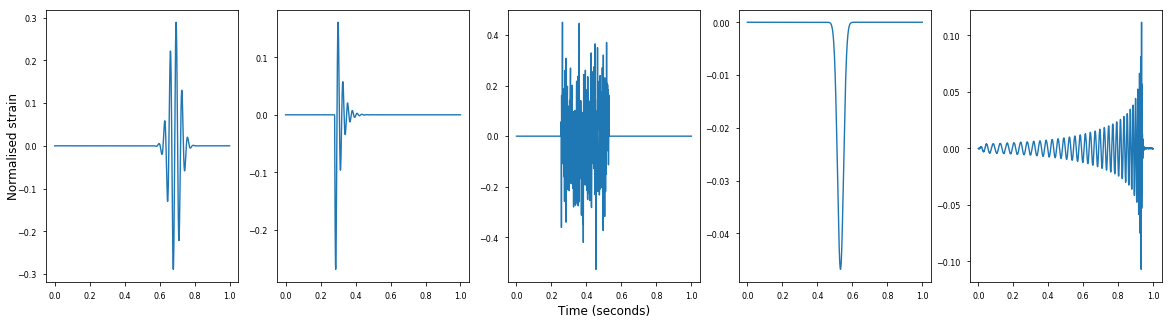
\includegraphics[width=\textwidth]{figures/train.png}
    \caption{Examples of burst training signals from left to right: sine-gaussian, ringdown, white-noise burst, Gaussian, binary-black hole merger}
    \label{fig:train}
\end{figure}

\subsection{Architecture details}
We base the architecture on (cite DCGANS) and adopt the suggestions of (cite wavegan paper) lengthening one-dimensional convolution kernels on both the generator and discriminator. The class label is interpreted as an additional channel early in the generator model. This is achieved by projecting the class inputs as a learned embedding layer, into a fully connected layer which can then be concatenated channel-wise to $\textbf{z}$. The rest of the model is fully convolutional, upsampled using strided transposed convolutions with batchnormalisation in the first layer and ReLU activations throughout with the exception of Tanh for the output layer. Each transposed convolutional layer uses a kernel size of 18x1 and stride 2.
The discriminator network mirrors that of the generator without batch normalization, using LeakyReLU activations, SpatialDropout, and a 2-stride convolution for downsampling. The main difference is that the discriminator has two output layers. The first output is a single node activated by a Sigmoid that can be interpreted as the realness of the the signal. The second output is 5 nodes activated using the softmax function predicting the class of the input. This model is trained with binary cross entropy for the first output and sparse categorical cross-entropy for the second output. \jordan{Diagram of generator with box and showing the concate procedure}

\subsection{Applying Antenna responses}
We consider a two detector case where the generator should be trained to output two identical signals with a physical time shift representing the time of flight between detectors and the suppression of amplitudes due to interaction with the detector. To achieve this, the generator is trained to generate a single waveform that is then manipulated through a non-trainable ``response" layer. This layer creates a copy of its input, shifts it along in time and applies antenna responses to both the input and shifted signal. The result is a 2x1024 times series waveform representing an overlay data stream from two detector outputs. 

%%%%%%%%%%%%%%%%%%%%%%%%%%%%%%%%%%%%%%%%%%%%%%%%%%%%%%%%%%%%%%%%%%%%%%%%%%%%%%
\section{Results}
%%%%%%%%%%%%%%%%%%%%%%%%%%%%%%%%%%%%%%%%%%%%%%%%%%%%%%%%%%%%%%%%%%%%%%%%%%%%%%

\begin{itemize}
\item Begin by outlining the type of results you will be presenting
\item A subsection on the general quality of generated waveforms - we may need
to have overlaps between generated wavefoms and training data (maybe)
\item A subsection on the descriminator - maybe a confusion matrix?
\item a subsection on the latent space varaition within each class - fixed
class, sliding in latent space.
\item A subsection on the class space variation - fixed latent space and
sliding in the class space.
\item A final subsection on the general waveform model based on random latent
and class space locations.
\item Make no conclusions.
\end{itemize}

\subsection{Waveform quality}
\begin{figure}
    \centering
    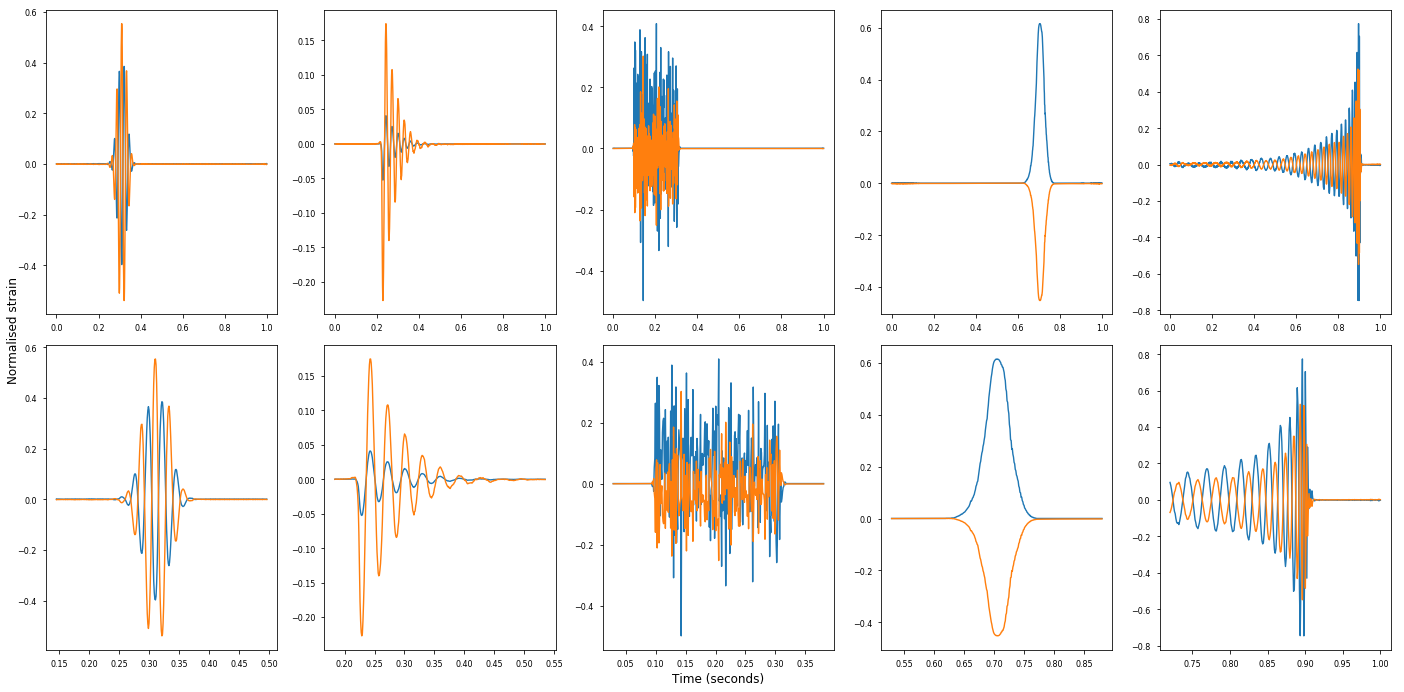
\includegraphics[width=\textwidth]{figures/gen_zoom_signals.png}
    \caption{Top row: Output of generator when given latent vector and class integer. Bottom row: Detailed view of the same output}
    \label{fig:gen_signals}
\end{figure}
\subsection{Classifier}
\subsection{Latent space interpolation}
\subsection{Class space interpolation}


%%%%%%%%%%%%%%%%%%%%%%%%%%%%%%%%%%%%%%%%%%%%%%%%%%%%%%%%%%%%%%%%%%%%%%%%%%%%%%
\section{Conclusions}
%%%%%%%%%%%%%%%%%%%%%%%%%%%%%%%%%%%%%%%%%%%%%%%%%%%%%%%%%%%%%%%%%%%%%%%%%%%%%%

\begin{itemize}
\item Summarise the paper
\item Dedicate a paragraph to each of the key results discussed in the previous
section
\item Have at least one paragraph on the future directions of this work
\item Conclude with a positive paragrpah about the potential uses and impact of
the approach.
\end{itemize}

\clearpage

\appendix
\section{List of hyperparameters}
\begin{table}[hb]
\caption{ACGAN architecture}
\footnotesize
\begin{tabular}{@{}lllllll}
\br
 Operation & Kernel & Strides & Output Shape & BN & Dropout & Activation \\
\mr
 G(\textbf{z}): Input \textbf{z} $\sim$ Normal(0,0.02) & N/A & N/A & (100,) & \ding{55} & 0 & N/A \\  
 Dense & N/A & N/A & (32768,) & \ding{55} & 0 & ReLU \\  
 Class input c & N/A & N/A & (1,) & \ding{55} & 0 & N/A \\
 Embedding & N/A & N/A & (1, 120) & \ding{55} & 0 & N/A \\
 Dense & N/A & N/A & (1,128) & \ding{55} & 0 & ReLU \\ 
 Reshape \textbf{z} & N/A & N/A & (128, 256) & \ding{55} & 0 & N/A \\
 Reshape c & N/A & N/A & (128, 1) & \ding{55} & 0 & N/A \\
 Concatenate & N/A & N/A & (128, 257) & \ding{55} & 0 & N/A \\
 Reshape & N/A & N/A & (64, 514) & \ding{55} & 0 & N/A \\
 Transposed Convolution & 18x1 & 2 & (256, 256) & \ding{51} & 0 & ReLU\\
 Transposed Convolution & 18x1 & 2 & (512, 128) & \ding{55} & 0 & ReLU\\
 Transposed Convolution & 18x1 & 2 & (1024, 64) & \ding{55} & 0 & ReLU\\
 Convolution & 18x1 & 1 & (1024, 1) & \ding{55} & 0 & Tanh \\
 Sky input & N/A & N/A & (3,) & \ding{55} & 0 & N/A \\
 Concatenate & N/A & N/A & (1027,) &  \ding{55} & 0 & N/A \\
 Lambda & N/A & N/A & (1024, 2) & \ding{55} & 0 & N/A \\
 D(\textbf{x}): Input \textbf{x} & N/A & N/A & (1024, 2) & \ding{55} & 0 & N/A \\
 Convolution & 14x1 & 2 & (512, 64) & \ding{55} & 0.5 & Leaky ReLU \\
 Convolution & 14x1 & 2 & (256, 128) & \ding{55} & 0.5 & Leaky ReLU \\
 Convolution & 14x1 & 2 & (128, 256) & \ding{55} & 0.5 & Leaky ReLU \\
 Convolution & 14x1 & 2 & (64, 512) & \ding{55} & 0.5 & Leaky ReLU \\
 Flatten & N/A & N/A & (32768,) & \ding{55} & 0 & N/A \\
 Dense & N/A & N/A & (1,) & \ding{55} & 0 & Sigmoid \\
 Dense & N/A & N/A & (5,) & \ding{55} & 0 & Softmax \\
\br
 Optimizer & \multicolumn{6}{l}{Adam($\alpha$ = 0.0002, $\beta_{1}$ = 0.5)} \\
 Batch size & \multicolumn{6}{l}{128}  \\
 Iterations & \multicolumn{6}{l}{60000}  \\
 Leaky ReLU slope & \multicolumn{6}{l}{0.2} \\
 Weight initialization & \multicolumn{6}{l}{Gaussian($\mu$ = 0, $\sigma$ = 0.02)} \\
 Generator loss & \multicolumn{6}{l}{Binary cross-entropy} \\
 Discriminator loss & \multicolumn{6}{l}{Binary cross-entropy \& sparse categorical cross-entropy} \\ 
 \br
\end{tabular}\\

\end{table}
\normalsize

\end{document}

